\setchapterpreamble[u]{\margintoc}
\chapter{Մոտարկում և ինտեգրում}
\labch{approx_integration}

\emergencystretch 2em

\section{Թեյլորի բազմանդամ}

Սովորաբար երբ փորձում են, ասենք, վերականգնել մեքենայի կամ ինքնաթիռի շարժման հետագիծը, վերցնում են ժամանակի ինչ-որ պահի (ասենք՝ շարժումը սկսելուց $t=2$ վ անց) նրա ունեցած դիրքը, արագությունը, արագացումը, արագացման արագությունը, և այլն, ու փորձում այդ թվերի միջոցով %\marginnote{ընդ որում՝ ինչքան շատ տվյալ ունե\-նանք, այնքան ճշգրիտ կվերականգնենք}
հաշվել, թե որ կետում կգտնվի մարմինը ենթադրենք՝ $t=3$ պահին։

Նույն ձևով՝ եթե ունենք որևէ $a$ կետում ինչ-որ մի անհայտ $f$ ֆունկցիայի արժեքը, ածանցյալը, երկրորդ կարգի ածանցյալը, և այլն, ապա կարող ենք մոտավորապես վերականգնել այդ $a$ կետի մոտակայքում $f$-ի ունեցած արժեքներն ու նրա գրաֆիկը։ Ինչպե՞ս դա անենք։

\question{Որքա՞ն են $f(x) = 10 + 5(x-3)$ ֆունկցիայի արժեքն ու ածանցյալը $x=3$ կետում։}

\begin{marginfigure}
    \centering
    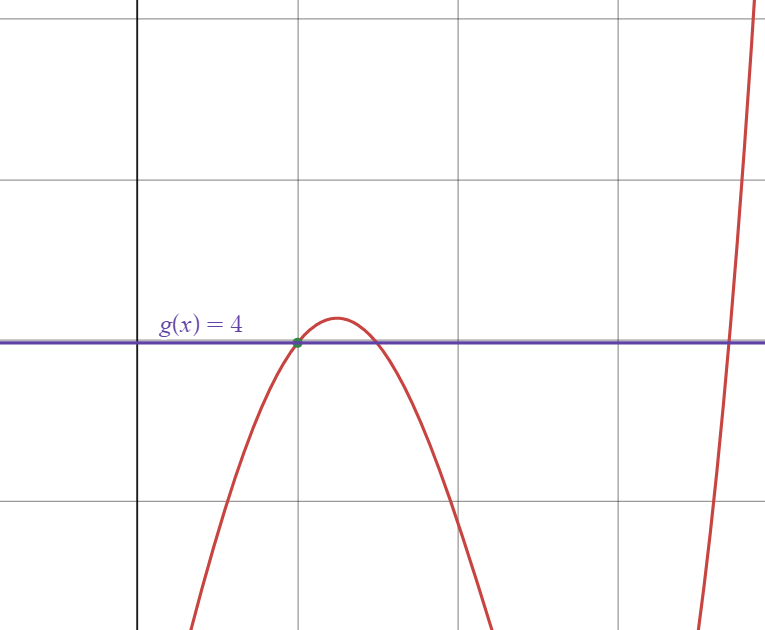
\includegraphics[width=\linewidth]{chapters/chapter 6/Taylor_1.1.png}
\end{marginfigure}

Ենթադրենք՝ ունենք, որ $f(a)=4$ և $f'(a)=3$։ Սկզբի համար կարող ենք վերցնել, ասենք, 
\[
g(x)=4  
\] 
ֆունկցիան, և այն $a$ կետում իր արժեքով հավասար կլինի $f$-ին՝ $g(a)=f(a)$։ Որպեսզի հավասարացնենք նաև $a$ կետում $f$-ի և $g$-ի ունեցած արագությունները, $g$-ին գումարենք այնպիսի բան, որի ածանցյալը $3$ է (օրինակ՝ $3x$), բայց որը գումարելով $g$-ի արժեքը չենք փչացնի (այսինքն՝ կշարունակենք ունենալ $f(a)=g(a)$)։ Գումարելով $3(x-a)$՝ կստանանք
\[
g(x)=4+3(x-a)
\]

Իրոք, եթե ստացված ֆունկցիան ածանցենք, կունենանք՝ $g'(a)=3$, ուրեմն՝ $g(a)=f(a)$ և $g'(a)=f'(a)$․ մեր սարքած $g$ ֆունկցիայի և՛ արժեքը, և՛ ածանցյալը համընկնում են $f$-ինի հետ։ Իհարկե, սա դեռ չի նշանակում, որ $f$-ն ու $g$-ն նույն ֆունկցիաներն են․ միգուցե ասենք՝ երկրորդ կարգի ածանցյալով դրանք իրարից տարբերվեն ($f''(a)\ne g''(a)$) և նույնը չլինեն։ Բայց երկրորդ կարգի ածանցյալի արժեքը (արագացումը) սովորաբար զգացվում է, երբ $a$ կետից փոքր-ինչ հեռանում ես, մինչդեռ եթե մենք շատ-շատ մոտ մնանք $a$ կետին, ապա $g$-ի արժեքները ու գրաֆիկը մոտավորապես նույնը կլինեն, ինչ $f$-ինը՝ 
\[
g(x) \approx f(x) \qquad \text{երբ $x$-ը շատ մոտ է $a$-ին}
\]

\begin{marginfigure}
    \centering
    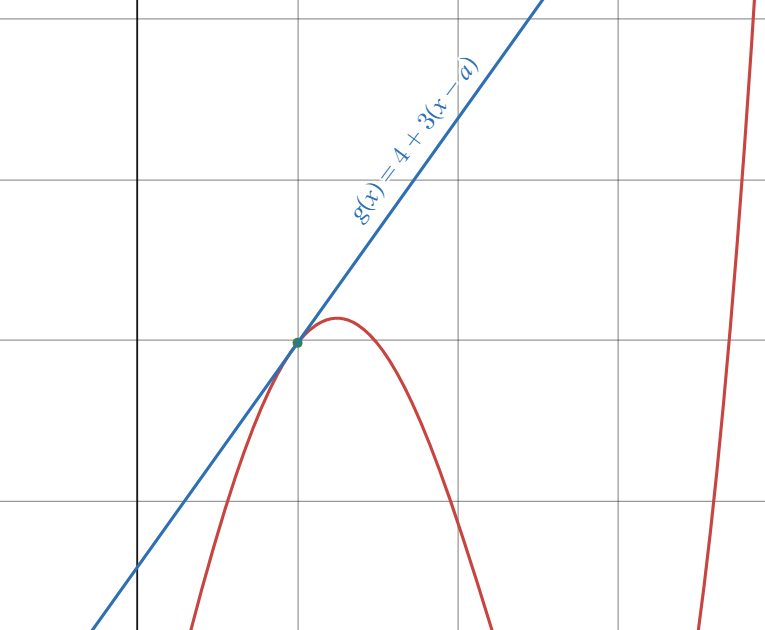
\includegraphics[width=\linewidth]{chapters/chapter 6/Taylor_1.2.png}
\end{marginfigure}

այլ կերպ ասած՝ մեր ստացած $g$ ֆունկցիան \textit{մոտարկում է} $f$-ին (թեև ոչ այնքան ճշգրիտ կերպով)։

Եթե ուզում ենք, որ այն ավելի ճշգրիտ մոտարկի, գնանք մեկ այլ առաջ․ փորձենք կառուցել այնպիսի $g$, որի արագացումը նույնպես համընկնի $f$-ինի հետ։ Ենթադրենք՝ $f''(a)=5$։

\question{Ի՞նչ գումարենք $g(x)$-ին, որպեսզի դրա երկրորդ կարգի ածանցյալը նույնպես $a$ կետում լինի $5$՝ $g''(a)=5$:}

Երկրորդ կարգի ածանցյալը ստանալու համար ավելացնենք ևս մեկ գումարելի՝
\[
g(x)=4+3(x-a)+\frac{5}{2}(x-a)^2
\]

\begin{marginfigure}
    \centering
    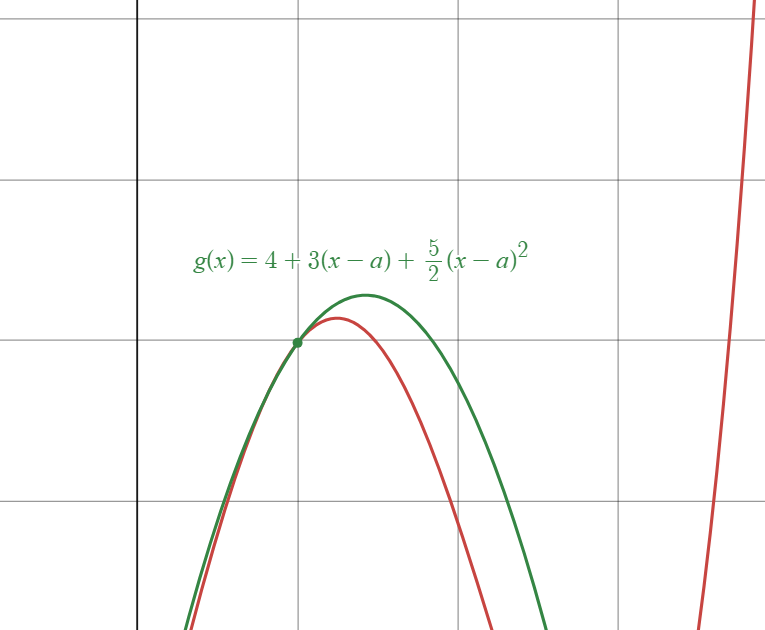
\includegraphics[width=\linewidth]{chapters/chapter 6/Taylor_1.3.png}
\end{marginfigure}

Կրկին, դժվար չէ ստուգել, որ այս ֆունկցիայի համար $g''(a)=f''(a)=5$ և $g(a)=f(a)$, $g'(a)=f'(a)$: Ինչո՞ւ ենք բազմապատկում $\dfrac{1}{2}$-ով․ որպեսզի ածանցելիս $(x-a)^2$-ու ցուցիչը իջնելով բազմապատկվի և կրճատվի դրա հետ (հակառակ դեպքում $g''(a)$-ն $2$ անգամ մեծ կլիներ)։

Այս սխեմայով եթե շարունակենք, կստանանք հետևյալ ֆունկցիան՝
\[
g(x) = f(a) + f'(a)\cdot (x-a) + \frac{f''(a)}{2}\cdot (x-a)^2 + \frac{f'''(a)}{3 \cdot 2}\cdot (x-a)^3 + \dots
\]
որը $a$ կետում կունենա
\begin{itemize}
    \item նույն արժեքը, ինչ $f$-ը
    \item նույն արագությունը, ինչ $f$-ը
    \item նույն արագացումը, ինչ $f$-ը
    \item նույն արագացման արագությունը, ինչ $f$-ը
    \item \dots 
\end{itemize}
հետևաբար բավական մոտ կլինի իսկական $f$ ֆունկցիայի արժեքներին $a$ կետի շրջակայքում։ Քանի որ գործնականում ոչ հնարավոր է, ոչ էլ կարիք կա հաշվելու բոլոր (անվերջ քանակով) ածանցյալները, սովորաբար բավարարվում են գրելով միայն առաջին մի քանի գումարելիները՝
\begin{align*}
P_k(x) &= f(a) + f'(a)\cdot (x-a) + \frac{f''(a)}{2}\cdot (x-a)^2 \\&+ \dots +
 \frac{f^{(k)}(a)}{k \cdot (k-1) \cdot \dots \cdot 2}\cdot (x-a)^k 
 = \sum_{j=1}^k \frac{f^{(j)}(a)}{j!}(x-a)^j
\end{align*}
և ստացված ֆունկցիան անվանում \textit{$k$-րդ կարգի \href{https://en.wikipedia.org/wiki/Taylor_Swift}{Թեյլորի} բազմանդամ։}

\begin{theorem}
Եթե $f(x)$ ֆունկցիան $k$ անգամ դիֆերենցելի\marginnote{$k$ անգամ դիֆերենցելի $=$ ունի $1$-ին, $2$-րդ, $\dots$, $k$-րդ կարգի ածանցյալներ} է $a$ կետում, ապա
\[
P_k(x) \approx f(x)
\]
$a$ կետի ինչ-որ (միգուցե՝ փոքր) շրջակայքում։ Ավելի \marginnote[*+2]{ի՞նչ կլինի, եթե օրինակ $x-a=0.1$, $k=5$}ճշգրիտ՝
\[
P_k(x) - f(x) = c \cdot (x-a)^{k+1}
\]
որտեղ $c$-ն ինչ-որ ֆիքսված թիվ է (արժեքը կարևոր չէ)։
\end{theorem}

\question{Կարո՞ղ եք գտնել $f(x)=x^2+7x-6$ ֆունկցիայի $10$-րդ կարգի Թեյլորի բազմանդամը։ Իսկ ո՞րն է դրա $2$-րդ կարգինը։ Իսկ $1$-ի՞ն։}

Այսինքն՝ որքան $k$-ն՝ գումարելիների թիվը, մեծացնենք, այնքան ավելի ճշգրիտ մոտարկում կստանանք $a$ կետին մոտիկ կետերում։ Համոզվելու համար \href{https://math.libretexts.org/Learning_Objects/Interactive_Calculus_Activities/Power_Series_1_Over_1-x}{տեսեք}, օրինակ, $\dfrac{1}{1-x}$ ֆունկցիայի Թեյլորի բազմանդամները։ Գործնականում հաճախ վերցնում են ընդամենը առաջին $k=1$ (գծա\-յին), $2$ (քառակուսային) կամ $3$ (խորանարդային մոտարկումներ) գումա\-րե\-լի\-ները․ մի կողմից դրանք բավարար ճշգրիտ են, մյուս կողմից՝ ավելի մեծ $k$-երի դեպքում ունենում ենք բարձր աստիճանի բազմանդամ, որը $a$-ից հեռու կետերում իրեն \marginnote{լավ չի պահում $=$ շատ է տատանվում}լավ չի պահում։

\warning{Նույն ֆունկցիայի համար, սակայն տարբեր $a$ կե\-տե\-րում գրված Թեյլորի բազմանդամները տարբերվում են։ Յուրաքանչյուրը լավ է մոտարկում միայն իր $a$ կետին մոտիկ տեղամասում, $a$-ից հեռանալիս՝ ճշգրտությունն ընկնում է։}

\begin{example}
$a=0$ կետի համար հետևյալ ֆունկցիաները կարելի է գրել՝
\begin{itemize}
\item $\displaystyle e^x = \sum_{n=0}^{\infty} \dfrac{x^n}{n!} = 1 + x + \dfrac{x^2}{2!} + \dfrac{x^3}{3!} + \cdots$

\item $\displaystyle \dfrac{1}{1-x}= \sum_{n=0}^\infty x^n = 1+x+x^2+x^3+x^4+\cdots $

\item $\displaystyle\ln(1+x)=\sum_{n=0}^\infty(-1)^n\dfrac{x^{n+1}}{n+1}=x -
\dfrac{x^2}{2} + \dfrac{x^3}{3} - \dfrac{x^4}{4}+ \cdots$

\item եթե $f$-ն ինքը բազմանդամ է, ապա $P_k$-ն նրա առաջին $k$ անդամներն են
\end{itemize} 
\end{example}

\question{Օգտվելով $\dfrac{1}{1+x}$-ի Թեյլորի բազմանդամից՝ ինչպե՞ս ստա\-նանք  $\dfrac{1}{1-x}$-ի Թեյլորի բազմանդամը։ }


\section{Անորոշ ինտեգրալ}

Ֆունկցիայի Թեյլորի բազմանդամը կառուցելիս առնչվեցինք նման հարցի․ ո՞ր ֆունկցիայի ածանցյալն է հավասար $3$-ի։ Քանի որ գիտեինք, թե ինչի են հավասար մի քանի տարբեր ֆունկցիաների ածանցյալները, հետ գնալով կռահեցինք, որ այդպիսի ֆունկցիա է $3x$-ը։

\question{Ո՞ր ֆունկցիայի ածանցյալն է $4x^3$։}

Ընդ որում $3x$-ից բացի նույն ածանցյալն ունեն նաև $3x+1$, $3x+4$, $3x-1000$ ֆունկցիաները։ Պատճառն այն է, որ երբ $3x$-ին գումարում ենք որևէ հաստատուն թիվ՝ $c$, վերջինիս ածանցյալը զրո է։ Ուրեմն $3x+c$ տեսքի բոլոր ֆունկցիաների ածանցյալները հավասար են $3$ ֆունկցիային։

Կարճ կասենք, որ եթե
\[
f\text{-ը }F\text{-ի ածանցյալն է}
\]
ապա
\[
F\text{-ը }f\text{-ի \textbf{նախնականն} է}
\]
իսկ $F$ ֆունկցիայի բոլոր նախնականները իրար հետ (բոլոր նախնա\-կան\-ների բազմությունը) կանվանենք $F$-ի \textit{անորոշ ինտեգրալ։} 

Փաստորեն ֆունկցիայի նախնականը այն ֆունկցիան է, որը պատաս\-խա\-նում է «ո՞ր ֆունկցիան ածանցեմ, որպեսզի ստանամ այս ֆունկցիան» հարցին, և բավարար է գտնել նմանատիպ որևէ ֆունկցիա ու դրան հաստատուն թվեր գումարելով՝ կստանանք մնացած բոլոր նախնական\-ները։

\begin{theorem}
$f$ ֆունկցիայի բոլոր նախնականներն իրարից տար\-բեր\-վում են հաստատուններով։
\end{theorem}

\begin{example}
$f(x)=4x^3$ ֆունկցիայի համար նախնական են
\begin{itemize}
    \item $x^4$
    \item $x^4+5$
    \item $x^4+100000000$
    \item $\dots$
\end{itemize}
ֆունկցիաները, այսինքն $f(x)$-ի բոլոր նախնականներն ունեն հետևյալ տեսքը՝ \marginnote{որտեղ $c$-ն ցանկացած հաստատուն է}
\[
x^4 + c
\]
\end{example}

$f(x)$-ի բոլոր նախնականները, նույն ինքը՝ անորոշ ինտեգրալը, կնշանակենք այսպես՝
\[
\int f(x) \, dx
\]
տվյալ օրինակում՝
\[
\int 4x^3 \, dx = x^4 + c
\]

Այս $\int$-ն ու $dx$-ը ընդամենը ինչ-որ սիմվոլներ են (ոչ մի բազմապատկում կամ այլ իմաստ չկա), որոնց արանքում գրում ենք մեր ինտեգրվող ֆունկցիան։ 

\question{Ո՞ր ֆունկցիան է և՛ ինքը իր նախնականը, և՛ ածանցյալը։}

Ինտեգրալը նույնպես օժտված է գծային հատկություններով․\marginnote[*+2]{$a$-ն ցանկացած թիվ է}
\begin{align*}
\int a \cdot f(x) \,dx &= a \cdot \int  f(x) \,dx
\\\int f(x) \pm g(x) \,dx &= \int f(x) \,dx \pm \int g(x) \,dx
\end{align*}

Եթե երկու ֆունկցիաների գումարը ինտեգրելիս դրանց որոշում ենք առանձին-առանձին ինտեգրել, յուրաքանչյուրի ինտեգրալը հաշվելիս ունենում ենք $+c$: Արդյունքում գումարի մեջ ունենում ենք $+2c$, որը սակայն կարող ենք գրել պարզապես $+c$․ այս $c$-երը կարող են լինել ցանկացած թվեր, և տարբերություն չկա՝ \marginnote{այսինքն՝ կարող ենք գրել \[\int 3x^2 + 4x \, dx = x^3 + 2x^2 + c\]} վերցնել ցանկացած թվին գումարել մեկ ուրիշ ցանկացած թիվ, թե՞ պարզապես վերցնել ինչ-որ մի երրորդ ցանկացած թիվ։

\question{Կարո՞ղ եք գտնել $\int \cos x \, dx$-ը։ Իսկ $\int 2x \cos (x^2)\, dx$-ը՞:}

Հիշենք երկու ֆունկցիաների արտադրյալի ածանցման կանոնը՝ 
\[
(fg)'=f'g+fg'
\]

Եթե մեզ պետք լիներ ստանալ ասենք՝ աջ մասի երկրորդ գումարելիի ինտեգրալը, կարող էինք նախ այն գրել այս տեսքով՝
\[
f(x)g'(x) = \underbrace{(f(x)g(x))'}_{\text{ո՞րն է նախնականը}} - f'(x)g(x)
\]
ապա երկու կողմերն ինտեգրել՝
\[
\int f(x)g'(x) \, dx = f(x)g(x) - \int f'(x)g(x) \, dx
\]

Այս բանաձևը հաճախ է օգտագործվում ինտեգրալներ հաշվելիս և կոչվում է \textit{մասերով ինտեգրում։} Հաճախ $g'(x)\,dx$-ի փոխարեն կարճ գրում են՝ $dg(x)$․
\[
\int f(x)g'(x) \, dx = \int f(x)\, dg(x)
\]
Նույն ձևով գրելով $f'(x)\, dx = df(x)$՝ կունենանք
\[
\int f\, dg = fg - \int g\, df
\]

\begin{marginfigure}
    {\centering \@setfontsize\Huge{30}{60}\[\int \]}
    \caption*{ինտեգրալը կիրառվում է նաև \href{https://youtu.be/o4-3_JoXiVU?feature=shared&t=481}{կյանքում}}
\end{marginfigure}

\begin{example}
Ո՞ր ֆունկցիայի ածանցյալն է $x\cos x$-ը։ Գրենք՝
\[
\int x \cos x\, dx 
\]
ներկայացնենք $\cos x$-ը որպես մեկ ուրիշ ֆունկցիայի ածանցյալ՝ 
\[
=
\int x (\sin x)'\, dx 
=
\int x \,d (\sin x)
=
x \sin x-\int \sin x\, dx
\]
իսկ այստեղ արդեն գիտենք, թե ով է $\sin x$-ի ինտեգրալը․
\[
=
x \sin x-\int \sin x\, dx
= 
x \sin x + \cos x + c
\]
Համոզվելու համար կարող ենք ստացվածը ածանցել և տեսնել, որ իրոք լինում է $x \cos x$: 
\end{example}

\question{Ո՞ր ֆունկցիաներն են $x^{100}$-ի նախնականները։}

Առայժմ ինտեգրելը խաղի նման ինչ-որ բան է՝ վերցնում ես ֆունկցիան, կռահում, թե ում ածանցյալն է։ Շուտով կպարզենք, թե ո՞րն է դրա կիրառական նշանակությունը։ Մինչ այդ ֆիքսենք մի քանի հայտնի ֆունկցիաների անորոշ ինտեգրալները՝
\begin{itemize}
\item $\displaystyle \int a \, dx= ax+c$
\item $\displaystyle \int x \, dx= \dfrac{x^2}{2}+c$
\item $\displaystyle \int x^n \, dx= \dfrac{x^{n+1}}{n+1}+c$ (բացառությամբ երբ $n=-1$)
\item $\displaystyle \int \dfrac{1}{x} \, dx= \int x^{-1} \, dx= \ln|x| + c$
\item $\displaystyle \int e^x \, dx= e^x+c$
\item $\displaystyle \int \cos x \, dx= \sin x+c$
\item $\displaystyle \int \sin x \, dx= $ լրացրու ինքդ
\end{itemize}

\question{Եթե ածանցյալը ֆունկցիայի արագությունն է, ապա ի՞նչ եք կարծում, ինտեգրա՞լն ինչը պիտի լինի։}

\section{Որոշյալ ինտեգրալ}

Նկարում պատկերված է մեքենայի արագության գրաֆիկը՝ կախված ժամանակից: Ինչպես հայտնի է, երբ մեքենան շարժվում է հավասարաչափ արագությամբ, նրա անցած ճանապարհը հավասար է ժամանակ $\times$ արագություն, այսինքն՝ $t \in [0, 10]$ միջակայքում մեքենայի անցած\marginnote{կարող ենք համարել՝ $v(t)=s'(t)$} ճանապարհը $= 100$ մ $=$ քառակուսի մասի մակերեսին։

\begin{figure}[h]
    \centering
    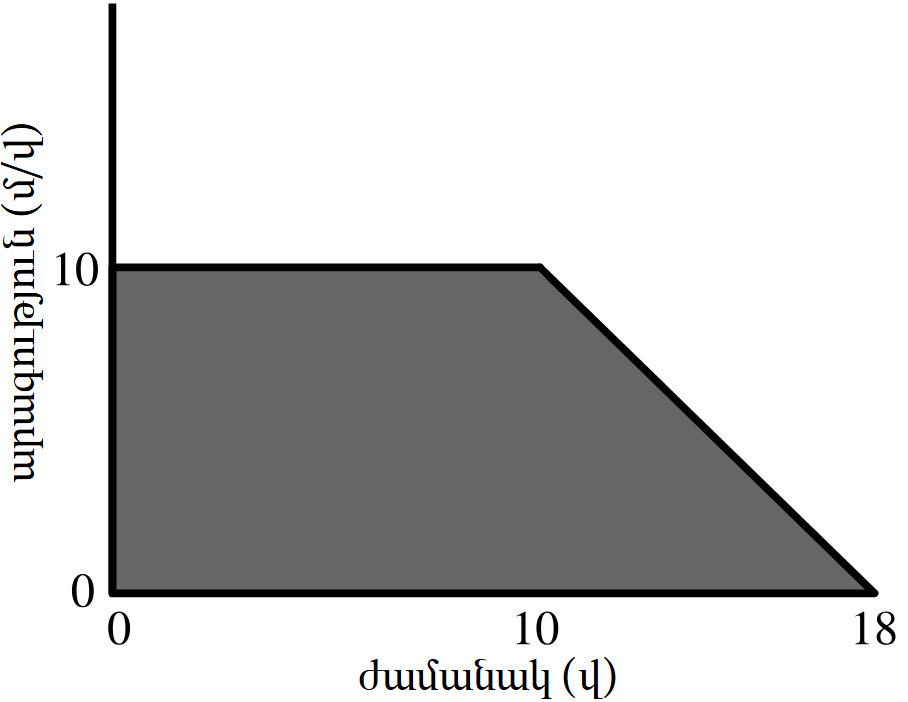
\includegraphics[width=0.6\linewidth]{chapters/chapter 6/velocity.png}
\end{figure}

$t=10$ պահից սկսած մեքենայի արագությունը սկսում է հաստատուն արագացմամբ նվազել և ի վերջո դառնում է $0$։ Ուրեմն $t \in [10, 18]$ միջակայքում մեքենայի միջին արագությունն է $5$, հետևաբար նրա անցած ճանապարհը $= 40$ մ $=$ եռանկյուն մասի մակերեսին։

Ինչպես նկատում եք, կա օրինաչափություն․ մարմնի անցած ճանապարհը յուրաքանչյուր $t\in [a, b]$ ժամանակահատվածում հավասար է $t=a$ և $t=b$ կետերի միջև նրա արագության գրաֆիկի տակ եղած մակերեսին։ Այս սկզբունքը ճիշտ է ոչ միայն հաստատուն կամ հավասարաչափ դանդաղող շարժման, այլ առհասարակ ցանկացած շարժման դեպքում։

\question{$s(t)$ ֆունկցիայի ի՞նչն է $v(t)$-ն։ Իսկ $v(t)$-ի ի՞նչն է $s(t)$-ն։}

Իսկ ի՞նչ, եթե արագության գրաֆիկը բաղկացած լիներ ոչ թե քառակու\-սուց և եռանկյունից, այլ լիներ ավելի բարդ տեսքի։ Ինչպե՞ս հաշվել այս կամ այն ֆունկցիայի գրաֆիկի տակ եղած մակերեսը։

\begin{figure}[t]
\centering %
\floatsetup{floatrowsep=qquad}
\begin{floatrow}[3]%
\ffigbox[\FBwidth]{}{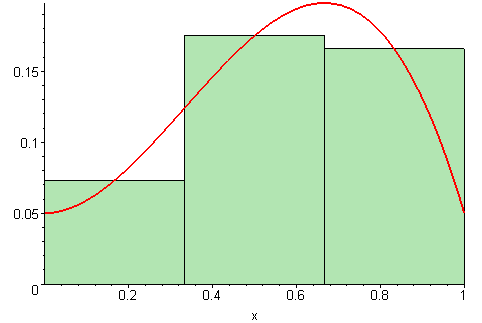
\includegraphics[width=0.4\textwidth]{chapters/chapter 6/Riemann 1.png}}
\ffigbox[\FBwidth]{}{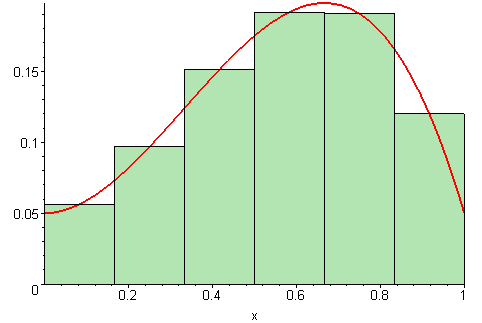
\includegraphics[width=0.4\textwidth]{chapters/chapter 6/Riemann 2.png}}
\ffigbox[\FBwidth]{}{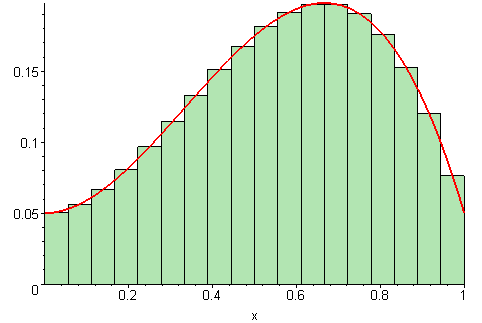
\includegraphics[width=0.4\textwidth]{chapters/chapter 6/Riemann 3.png}}
\end{floatrow}
\end{figure}

% \begin{figure}[h]
%     \centering
%     \subfloat{{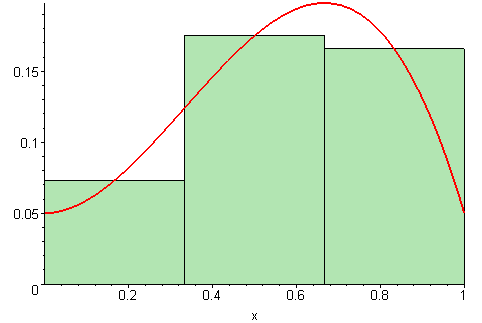
\includegraphics[width=0.3\linewidth]{chapters/chapter 6/Riemann 1.png} }}%
%     \quad
%     \subfloat{{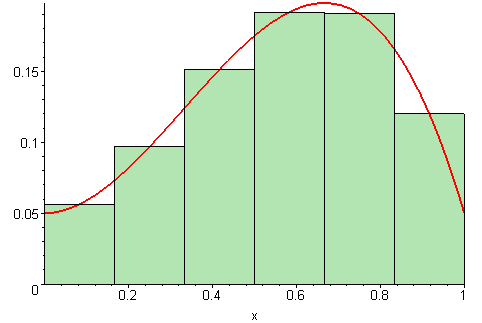
\includegraphics[width=0.3\linewidth]{chapters/chapter 6/Riemann 2.png} }}%
%     \quad
%     \subfloat{{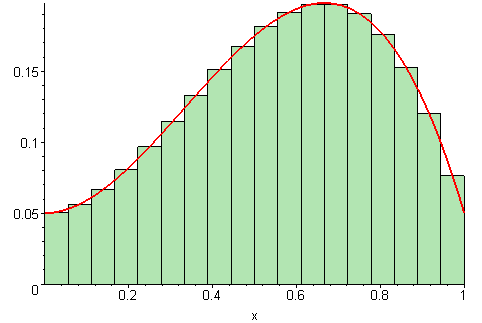
\includegraphics[width=0.3\linewidth]{chapters/chapter 6/Riemann 3.png} }}%
% \end{figure}

Ինչպես և հավանաբար կանեիք առօրյա կյանքում, մոտարկենք այդ մակերեսը \textit{ուղղանկյուններով․} բաժանենք մեր $[a, b]$ միջակայքը (տրոհենք) բազ\-մա\-թիվ փոքր հատվածիկների՝\marginnote[*+1.9]{որտեղ $x_0=a$, իսկ $x_n=b$}
\[
[x_0, x_1],\quad [x_1, x_2],\quad \dots, \quad [x_{n-1}, x_n]
\]
յուրաքանչյուր $k$-րդ հատվածի չափը նշանակելով $\Delta x_k$-ով՝ $\Delta x_k = x_{k}-x_{k-1}$, այնուհետև յուրաքանչյուր հատվածի վրա կառուցենք այնպիսի ուղղանկյուն, որը մոտիկ լինի այդ հատվածի վրա $f$-ի գրաֆիկին։ Քանի որ $f$-ի գրաֆիկի «բարձրությունը» պարզապես ամեն կետում $f$-ի ընդունած արժեքն է, ամեն $[x_{k-1}, x_k]$ հատվածում վերցնենք որևէ $c_k$ կետ և դիտարկենք այն ուղղանկյունը, որի
\begin{itemize}
    \item բարձրությունը $f(c_k)$ է
    \item հիմքը՝ $[x_{k-1}, x_k]$ հատվածը
\end{itemize}

Ստացված ուղղանկյան մակերեսը կլինի $f(c_k) \cdot \Delta x_k$, հետևաբար բոլոր ուղղանկյունների մակերեսը միասին՝
\[
\sum_{k=1}^{n} f(c_k)\, \Delta x_k
\]
Որքան $n$-ը մեծ լինի, իսկ հատվածիկների երկարությունները՝ փոքր, այնքան այս գումարը մոտ կլինի $f$-ի գրաֆիկի տակ եղածին։ Այն թիվը, \marginnote{$c_k$-երի ընտրությունը այստեղ կարևոր չէ, քանի որ վերջում \href{https://www.sfu.ca/math-coursenotes/Math\%20158\%20Course\%20Notes/sec_defint.html##:~:text=1.4.2}{նույն թիվն} ենք ստանալու (երբ $n \to \infty$)} որը կստանանք՝ վերևի գումարում հատվածների երկարությունները ձգտեցնելով $0$-ի, ցույց կտա $[a,b]$ միջակայքում $f$-ի գրաֆիկով սահ\-մա\-նա\-փակված մակերեսը և կկոչվի $f$ ֆունկցիայի \textit{որոշյալ ինտեգ\-րալ} այդ միջակայքում։

\begin{definition}
Հետևյալ թիվը՝ \marginnote{ավելի ճշգրիտ՝ ոչ թե  
$\lim\limits_{n \to \infty}$, այլ $\lim\limits_{\lambda \to 0}$, որտեղ $\lambda$-ն ամենաերկար հատվածի եր\-կա\-րու\-թյունն է
}
\[
\lim_{n \to \infty} \sum_{i=1}^n f(c_i) \,\Delta x_i
\]
կոչվում է $f(x)$ ֆունկցիայի \textbf{որոշյալ ինտեգրալ} $[a,b]$ միջակայքում և նշանակվում՝
\[
\int_a^b f(x)\, dx
\]
\end{definition}

\newpage
\begin{marginfigure}
\centering
\caption*{ասում են, որ $\int_a^b f(x)\,dx$-ը \textit{նշանափոխ} մակերես է ({\it signed} {\rm area})}
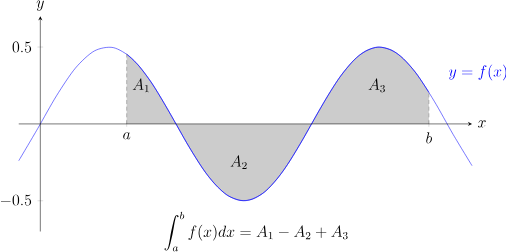
\includegraphics[width=\linewidth]{chapters/chapter 6/net area.png}
\end{marginfigure}Այստեղ անենք մի կարևոր նշում։ Եթե $f(x)$-ի արժեքները $[a,b]$ միջակայքում դրական են, այսինքն՝ նրա գրաֆիկը ընկած է $x$-երի առանցքից վերև, ապա $\int_a^b f(x)\,dx$-ը իրոք կտա դրանից ներքև եղած մակերեսը, բայց եթե այն բացասական է՝ $f(x) < 0$ ($x$-երի առանցքից ներքև), ապա $\int_a^b f(x)\,dx$-ի արժեքը կլինի \textit{բացասական՝} $f$-ի գրաֆիկի և $x$-երի առանցքի արանքում ընկած մակերեսը, սակայն մինուս նշանով։ Այսինքն կախված $[a,b]$-ում $f$-ի նշանից՝ դրա որոշյալ ինտեգրալը մոդուլով հավասար է նրա գրաֆիկով սահմանափակված մակերեսին, իսկ նշանով համընկնում է $f$-ի հետ։

\question{Որքա՞ն է $\int_a^b f(x)\,dx$-ը, եթե $f$-ը $[a,b]$ միջակայքում հավասար է $0$-ի։ Հնարավո՞ր է, որ $\int_a^b f(x)\,dx=0$, բայց $f$-ը $0$ չլինի։}

\section{Նյուտոն-Լայբնիցի բանաձևը}

Ինչպե՞ս հաշվել $\int_a^b f(x)\,dx$-ը, եթե ունենք $f(x)$-ի բանաձևը (կամ առհասարակ ինչո՞ւ է այն կոչվում «ինտեգրալ»)։ Օրինակ՝ երբ $f$-ը մարմնի արագությունն է, որը իր հերթին անցած ճանապարհի ածանցյալն է՝ ${f(t) = v(t) = s'(t)}$, ապա ${t=a}$ և ${t=b}$ կետերի միջև նրա գրաֆիկի տակ եղած մակերեսը այդ ընթացքում մարմնի անցած ճանապարհն է՝ $\int_a^b v(t)\, dt=s(b)-s(a)$։ Պարզվում է, որ այս կանոնը ճիշտ է ցանկացած դեպքում․

\begin{theorem}
Եթե $F(x)$ ֆունկցիան $f(x)$-ի որևէ նախնական է, ապա
\[
\int_a^b f(x)\,dx = F(b)-F(a)
\]
\end{theorem}

Այսինքն՝ ֆունկցիայի տակ եղած մակերեսը երկու կետերի միջև հավասար է այդ կետերի միջև իր նախնականի \textit{փոփոխությանը։} Ճիշտ է՝ $f$-ը ունի ոչ թե մեկ նախնական, այլ անվերջ հատ, \marginnote{եթե $G$-ն նույնպես $f$-ի նախնական է, ապա $G(x) = F(x) + c$, հետևաբար $$G(b)-G(a)=F(b)-F(a)$$} բայց դրանց բոլորի տարբերությունները երկու կետերի միջև նույնն են։ Ուրեմն՝ $\int_a^b f(x)\,dx$-ը հաշվելու համար հաշվում ենք (անորոշ) $\int f(x)\,dx$-ը, այսինքն՝ գտնում $f$-ի որևէ $F$ նախնական (տարբերություն չկա, թե որը), և հաշվում դրա արժեքների տարբերությունը $a$ և $b$ կետերում։

\begin{example}
\marginnote[*+1.5]{$F(b)-F(a)$ կարճ գրում ենք՝ $F(x)\big\vert_{x=a}^b$}$y=x^2$ պարաբոլի տակ եղած մակերեսը $x\in[0,2]$ միջա\-կայքում՝
\[
\left.\int_{0}^{2} x^2 \,dx = \frac{1}{3} \cdot  x^3\right|_{x=0}^{2} = \frac{1}{3} (2^3 - 0^3) = \frac{8}{3}
\]

Նույն կերպ $y=\sin x$-ինը $x\in [0, \pi]$-ում՝
\[
\left.\int_{0}^{\pi} \sin x \,dx =  -\cos x\right|_{x=0}^{\pi} = -\cos \pi - (-\cos0) = 2
\]

Նկատենք, որ $[0, \pi]$ միջակայքում սինուսը դրական է, այսինքն այն, ինչ ստացել ենք, հենց գրաֆիկի ներքևում եղած մակերեսն է։ Իսկ այ օրինակ՝ 
\[
\left.\int_{0}^{\pi} \cos x \,dx =  \sin x\right|_{x=0}^{\pi} = \sin \pi - \sin 0 = 0
\]
ոչ թե որովհետև կոսինուսի գրաֆիկի տակ մակերես չկա, այլ որով\-հետև $[0, \pi]$ միջակայքի առաջին կեսում ֆունկցիան դրական է, երկ\-րոր\-դում՝ բացասական, դրա հաշվին գումարը զրոյանում է։
\end{example}

\question{Ինչպե՞ս կհաշվեք $|\cos x|$-ի տակ եղած մակերեսը $[0, \pi]$-ում։}

Բնականաբար, որոշյալ ինտեգրալը նույնպես ունի այն գծային հատկություններն, ինչ անորոշը․
\begin{align*}
\int_{a}^{b} c \cdot f(x) \,dx &= c \cdot \int_{a}^{b} f(x) \,dx    
\\
\int_{a}^{b} f(x) \pm g(x) \,dx &= \int_{a}^{b} f(x) \,dx \pm \int_{a}^{b} g(x) \,dx
\end{align*}

Մյուս կողմից՝ ցանկացած $[a,b]$ միջակայքում եղած մակերեսը կարող ենք գրել որպես երկու մակերեսների գումար՝ $a$-ից $c$ և $c$-ից $b$․
\[
\int_{a}^{b} f(x) \,dx = \int_{a}^{c} f(x) \,dx + \int_{c}^{b} f(x) \,dx
\]

Կարող ենք նաև ավելի հեռուն գնալ և սահմանել ասենք՝ $\int_5^2 f(x)\,dx$, որպես $[2, 5]$ միջակայքում $f$-ի գրաֆիկով սահմանափակված մակերեսը՝ հակառակ նշանով․
\[
\int_{a}^{b} f(x) \,dx = -\int_{b}^{a} f(x) \,dx 
\]
և գրել նաև՝ $\int_{a}^{a} f(x) \,dx = 0$:

Վերջապես նկատենք մի այսպիսի նրբություն․ երբ գրում ենք $\int_a^b f(x)\, dx$, նկատի ունենք $f$ ֆունկցիայի գրաֆիկի տակի մակերեսը (համապատաս\-խան նշանով)։ Այդ մակերեսի արժեքի մեջ $x$ փոփոխականը որևէ դեր չի խաղում․ կարող էինք $x$-ի փոխարեն գրել, ասենք, $y$ կամ $z$՝
\[
    \int_4^{25} \sin x \, dx
    =
    \int_4^{25} \sin y \, dy
\] 
\begin{marginfigure}
\centering
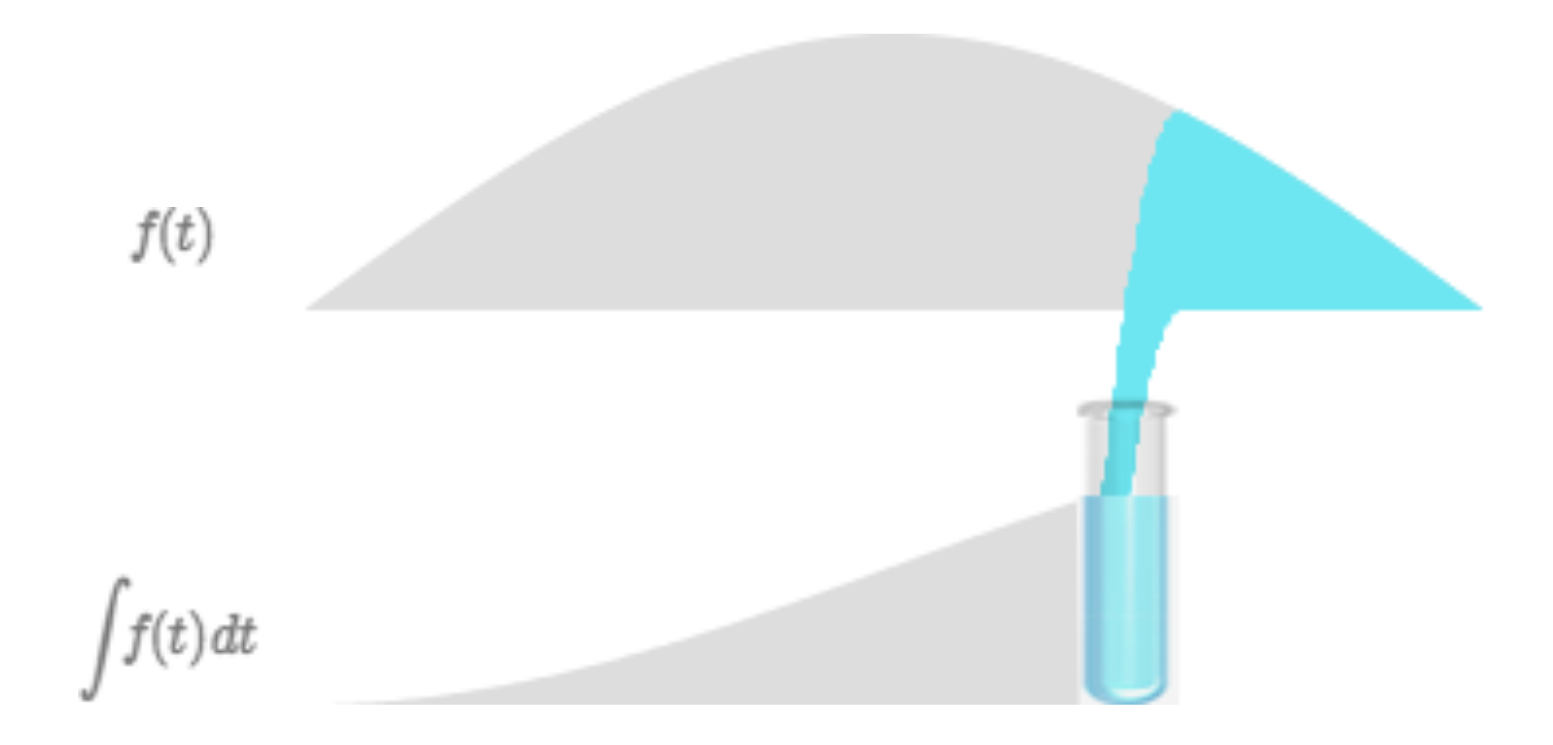
\includegraphics[width=\linewidth]{chapters/chapter 6/water filling.png}
\caption*{կամ՝ $t$-ն/$x$-ը/$y$-ը մեր բաժակն է, որը $a$-ից $b$ տանելով \href{https://worrydream.com/KillMath/#:~:text=little\%20tank\%20filling\%20up}{լցնում ենք} ջրով}
\end{marginfigure}
Պատկերավոր ասած՝ գծում ենք ֆունկցիայի գրաֆիկն ու ${y=4}$ կետից շարժվում դեպի ${y=25}$ կետը։ Ամեն կետում չափում ենք գրաֆիկի բարձրությունը, և որքան մեծ է ֆունկցիայի արժեքը, այնքան ավելի շատ մակերես ենք ստանում, որքան փոքր է՝ այնքան քիչ, իսկ բացա\-սա\-կան արժեքների դեպքում ստանում ենք բացասական մակերես։ Այս գործողության ընթացքում $y$-ը մեր պուլտն է, որով կառավարում ենք $4$-ից դեպի $25$ շարժը․ անկախ նրանից, թե ինչպես կանվանենք այդ պուլտը, ստացվող մակերեսը նույնն է։ Հետևաբար՝ ինտեգրելիս փոփոխականի անունը \textit{կարևոր չէ։}

Ավելին, կարող էինք նույնիսկ $y$-ի քառակուսի արմատը նշանակել $\sqrt{y}=t$-ով և $y$-ի փոխարեն գրել $t^2$՝ $\sin(t^2)\,d(t^2)$։ Միակ բանը, որին պետք է ուշադրություն դարձնենք, այն է, որ եթե $y$-ը փոխվում է $4$-ից $25$, ապա նրա արմատը՝ $t$-ն, պետք է փոխվի $\sqrt{4}$-ից $\sqrt{25}$, այսինքն՝
\[
\int_4^{25} \sin y \, dy = \int_2^5 \sin (t^2) \, d(t^2)
\]

\begin{example}
Հաշվենք $\dfrac{1}{x-4}$-ի գրաֆիկի տակ եղած մակերեսը $[5, 10]$ միջակայքում․
\[
\int_5^{10} \frac{1}{x-4}\, dx
\]

Ինչքան լավ կլիներ, եթե $x-4$-ի փոխարեն ունենայինք $x$։\marginnote{\hyperref[derivatives_list]{\color{OliveGreen}հիշենք}, որ $\dfrac{1}{x}$-ի նախնականը $\ln x$ է} Բայց այ եթե $x-4$-ը նշանակենք $y$-ով, կունենանք հենց $\dfrac{1}{y}$։ 

Եթե $x\in [5, 10]$, ապա $y\in [5-4, 10-4]$, այսինքն՝ $y\in [1, 6]$, և կունենանք՝
\[
\int_5^{10} \frac{1}{x-4}\, dx
=
\int_1^6 \frac{1}{y}\, d(y+4)
\]
Այստեղ \marginnote{ինչպես հիշում ենք, $dg(x) = g'(x)\,dx$} $d(y+4) = (y+4)' \, dy = 1 \cdot dy$, հետևաբար՝
\[
\int_1^6 \frac{1}{y}\, d(y+4)
=
\left.\int_1^6 \frac{1}{y}\, dy
= 
\ln y
\right|_{y=1}^6 
= 
\ln 6 - \ln 1 = \ln 6 \approx 1.79
\]
\end{example}

Այս մեթոդը կոչվում է \textit{փոփոխականի փոխարինում։}

\question{Ենթադրենք $f(x)$-ի գրաֆիկը համաչափ է սկզբնակետի նկատ\-մամբ, այսինքն՝ $f(-x)=-f(x)$։ Փորձեք պատկերել այդպիսի որևէ ֆունկցիայի գրաֆիկ։ Որքա՞ն է $\int_{-10}^{10} f(x)\, dx$-ը։}


\section{Ուռուցիկություն}

Եթե $1$-ին կարգի ածանցյալը ցույց է տալիս ֆունկցիայի արագությունը, ապա $2$-րդ կարգինը ցույց է տալիս նրա արագացումը։ Փորձենք երկրա\-չափորեն մեկնաբանել դա։

Նախ՝ ենթադրենք $f'(a)>0$, ուրեմն՝ $f$-ը $a$ կետում աճում է։ \marginnote[*+4]{ի՞նչ եք կարծում, ո՞ր գրաֆիկում է ֆունկ\-ցիայի արագացումը դրական}Բայց ֆունկցիան կարող է աճել տարբեր ձևերով, ասենք այսպես՝\newline
\begin{figure}[h]
    \centering
    $\vcenter{\hbox{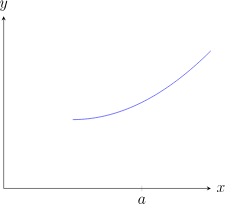
\includegraphics[width=0.3\linewidth]{chapters/chapter 6/convex.png}}}$%
    \hfill 
    կամ էլ այսպես՝
    \hfill
    $\vcenter{\hbox{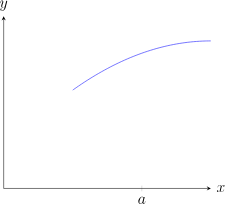
\includegraphics[width=0.3\linewidth]{chapters/chapter 6/concave.png}}}$
\end{figure}

պատկերավոր ասած՝ տակով կամ վրայով։ 

\begin{definition}
Եթե $(a,b)$ միջակայքի ցանկացած երկու կետերում ֆունկցիայի գրաֆիկն ընկած է այդ կետերը միացնող \marginnote{անգլերեն՝ ուռուցիկ — {\rm convex},\\ գոգավոր — {\rm concave}} հատվածից
\begin{itemize}
    \item ներքև, ապա կասենք, որ ֆունկցիան \textbf{ուռուցիկ} է $(a,b)$-ում
    \item վերև, ապա կասենք, որ ֆունկցիան \textbf{գոգավոր} է $(a,b)$-ում
\end{itemize}
\end{definition}

\begin{figure}[h]
    \centering
    
\includegraphics[width=0.8\linewidth]{chapters/chapter 6/convexity.png}
\end{figure}

Կետերը միացնող հատվածից վերև կամ ներքև գտնվելը կարող ենք ձևակերպել նաև այսպես․ ֆունկցիան\marginnote[*+3]{ի՞նչ է սա նշանակում $\alpha=0.5$ դեպքում}
\begin{itemize}
\item ուռուցիկ է, եթե
\[
f(\textcolor{myred}{\alpha } p + (\textcolor{myblue}{1-\alpha })q) \leq \textcolor{myred}{\alpha } f(p) + (\textcolor{myblue}{1-\alpha }) f(q)
\] 
\item գոգավոր է, եթե
\[
f(\textcolor{myred}{\alpha } p + (\textcolor{myblue}{1-\alpha })q) \ge \textcolor{myred}{\alpha } f(p) + (\textcolor{myblue}{1-\alpha }) f(q)
\]
\end{itemize}
ցանկացած $p, q \in [a,b]$ կետերի և $0 \le \alpha \le 1$ թվի դեպքում։

\warning{Ֆունկցիան կարող է մի կետում ուռուցիկ լինել, մյուսում՝ գոգավոր։}

Վերևում գրվածը չենք ապացուցի, բայց կզգանք, թե այն ինչ է նշա\-նա\-կում՝ \href{https://www.desmos.com/calculator/hx6weawigr}{բզբզալով} $\alpha$-ի արժեքները։ Ինչպես կռահում եք, ֆունկցիայի ուռուցիկ/գոգավոր լինելը կարելի է պարզել նրա երկրորդ կարգի ածանցյալի միջոցով․

\begin{theorem}
Եթե $f(x)$ ֆունկցիան երկու անգամ դիֆերենցելի է, ապա
\begin{itemize}
    \item $f$-ը ուռուցիկ է այն կետերում, որտեղ $f''(x) \ge 0$
    \item $f$-ը գոգավոր է այն կետերում, որտեղ $f''(x) \le 0$
\end{itemize}
\end{theorem}

\begin{example}
\\~
\begin{itemize}
\item $f(x) = x^2$-ն ուռուցիկ է բոլոր կետերում, քանի որ
\[
f''(x) = 2 > 0
\]
\item $f(x) = -x^2$-ն գոգավոր է բոլոր կետերում, քանի որ
\[
f''(x) = -2< 0
\]
\newpage
\item $f(x) = \sin x$-ը $(0, \pi)$ միջակայքում գոգավոր է, իսկ $(\pi, 2\pi)$-ում՝ ուռուցիկ․
\[
f''(x) = (\cos x)' = -\sin x
\]
\end{itemize}
\end{example}


\question{Ո՞ր ֆունկցիան է, որ ցանկացած կետում և՛ ուռուցիկ է, և՛ գոգավոր։}



\bigskip 

\begin{theory}
.
\begin{itemize}
\item կարդալ [{\rm Stewart}], 290-295 էջերը (ուռուցիկություն)
\item ըստ ցանկության՝ նաև [{\rm Stewart}], 325-328 էջերը
\item կարդալ [{\rm Banner}], 519-523 էջերը (Թեյլորի բազմանդամ)
\item վերադառնալ [{\rm Stewart}], 365-366, 372-373, 379-381, 391-394, 397-398 էջերին (ինտեգրալ)
\item ծանոթանալ [{\rm Stewart}]-ի 7-րդ գլխին (ինտեգրման մեթոդներ)
\item դիտել  {\rm 3b1b}-ի \href{https://www.3blue1brown.com/lessons/integration}{11-րդ} և \href{https://www.3blue1brown.com/lessons/taylor-series}{14-րդ} տեսադասերը մաթանալիզից 
\item ըստ ցանկության՝ նաև \href{https://www.3blue1brown.com/lessons/taylor-series-geometric-view}{15-րդը}
\item կարելի է նաև գտնել լուծված վարժություններ \href{https://tutorial.math.lamar.edu/Classes/CalcI/CalcI.aspx}{այստեղ}
\end{itemize}
\end{theory}

\newpage

\section{Խնդիրներ}


\begin{problem}
Գտեք $\displaystyle \int f(x)\, dx$-ը․
\begin{enumerate}[label={\alph*}․]
\item $f(x)=3x^2$
\item $f(x)=x+6\cos x$
\item $f(x)=\dfrac{3}{x}-1$
\item $f(x)=\dfrac{4x}{1-2x^2}$
\item $f(x)=\operatorname{tg}x$
\end{enumerate}
\end{problem}


\begin{problem}\marginnote[*+0.5]{\href{https://youtu.be/avDg6SmyMoY}{լուծում}}
Տիեզերանավը թռչում է Երկրից Լուսին։ Թռիչքի մեկնարկից $x$ ժամ անց նրա արագությունը
 \[f(x) = x^5+x^2\] 
հզր կմ/ժ է։
\begin{enumerate}[label={\alph*}․]
\item որքա՞ն ճանապարհ է այն անցնում առաջին $3$ ժամում
\item հետևաբար, որքա՞ն է տիեզերանավի միջին արագությունը
\end{enumerate}
\end{problem}


\begin{problem}\marginnote[*+0.5]{\href{https://youtu.be/EWhCu2C-d0M}{լուծում}}
Նկարում պատկերված է 
\[
f(x) = -x \cdot \ln (x^2)
\]
ֆունկցիայի գրաֆիկը $[0,1]$ հատվածի վրա։
\begin{figure}[h]
\centering
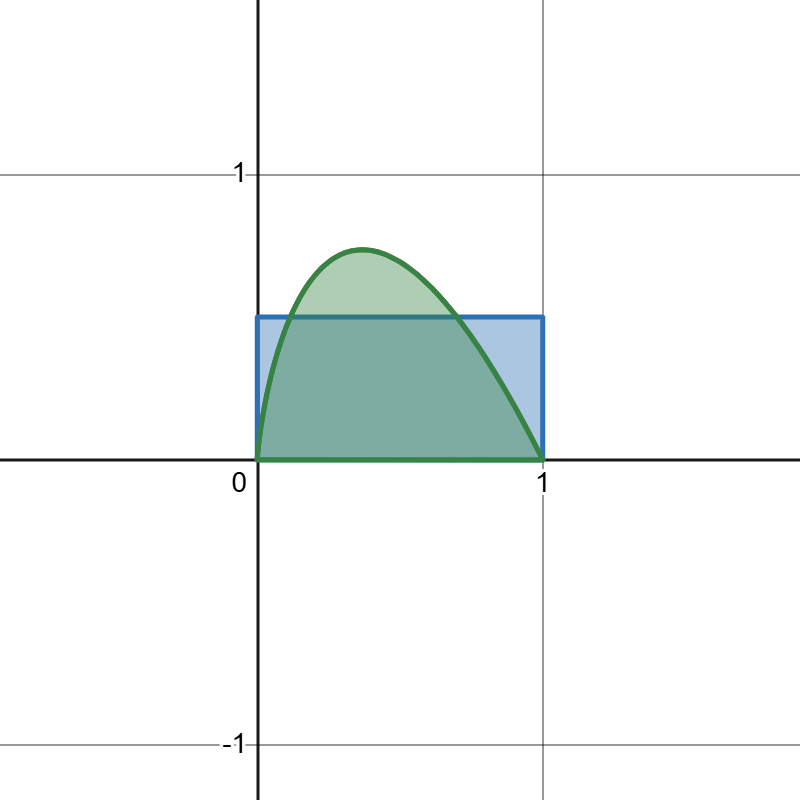
\includegraphics[trim={3cm 6cm 0 1cm},clip, width=0.5\linewidth]{chapters/chapter 6/equal_areas.png}
\end{figure}
Հայտնի է, որ կանաչ և կապույտ տիրույթներն ունեն նույն մակերեսը։
Որքա՞ն է կապույտ ուղղանկյան բարձ\-րությունը։
\end{problem}


\begin{problem}
Կան երկու ֆունկցիայից նոր ֆունկցիա ստանալու մի քանի տարբեր ձևեր։ Դրանցից մեկը, որ կարևոր դեր է խաղում մեքենայական ուսուցման մեջ, կոչվում է \textit{փաթույթ։}\marginnote[*+0.2]{անգլերեն՝ {\it convolution}}

Երկու $f$ և $g$ ֆունկցիաների փաթույթ է կոչվում (և $f*g$-ով նշանակվում) այն ֆունկցիան, որը որոշվում է հետևյալ բանաձևով՝\marginnote[*+2.4]{$x$-ը ֆիքսված է, $y$-ը փոփոխվում է}
\[
(f*g)(x) = \int_{-1}^1 f(y)g(x-y) \, dy
\]

Որքա՞ն է $f*g$-ի արժեքը $x=0$ կետում, եթե $f(x)=x^2$ և 
\[
g(x) = \begin{cases}
    1 & \text{եթե } x > 0 \\
    0 & \text{եթե } x \le 0
\end{cases}
\]

\hint{$f*g$-ում տեղադրեք $g$-ի բանաձևը, ապա բաժանեք $[-1, 1]$ միջակայքը երկու մասի՝ որտեղ որ $g=0$, և որտեղ $g=1$։}
\end{problem}


\begin{problem}
Պարզենք, թե որքան է $r$ շառավղով շրջանի մակերեսի բանաձևը։ Սկսենք $1$ շառավղով շրջանից՝ $x^2+y^2=1$։
\begin{enumerate}[label={\alph*}․]
\item արտահայտեք $y$-ն $x$-ով, ո՞ր միջակայքում է փոխվում $x$-ը
\item ո՞ր $f(x)$ ֆունկցիայի ինտեգրալն է պետք հաշվել
\item կատարեք փոփոխականի փոխարինում՝ $x$-ը նշանակելով $\sin t$-ով, ո՞ր միջակայքում պետք է փոփոխենք $t$-ն
\item ի՞նչ արտահայտություն է ստացվում ինտեգրալի նշանի տակ
\item օգտվելով $(\cos t)^2=\dfrac{1+\cos(2t)}{2}$ բանաձևից՝ հաշվեք ինտեգրալը
\item որքա՞ն է $1$ շառավղով շրջանի մակերեսը
\item ի՞նչ գծային ձևափոխություն կիրառենք՝ $r$ շառավղով շրջան ստանալու համար
\item քանի՞ անգամ կմեծանա մակերեսը
\end{enumerate}
\end{problem}
